\section{\pretty{Casa-nlu}: Context-Aware Self-Attentive NLU}
\label{sec:cdisan_f}
Our model architecture is composed of three sub sections - signal encoding, context fusion and IC-SL predictions (Figure \ref{cSA}).
\vspace{-10pt}
\begin{figure}[ht]
\centering
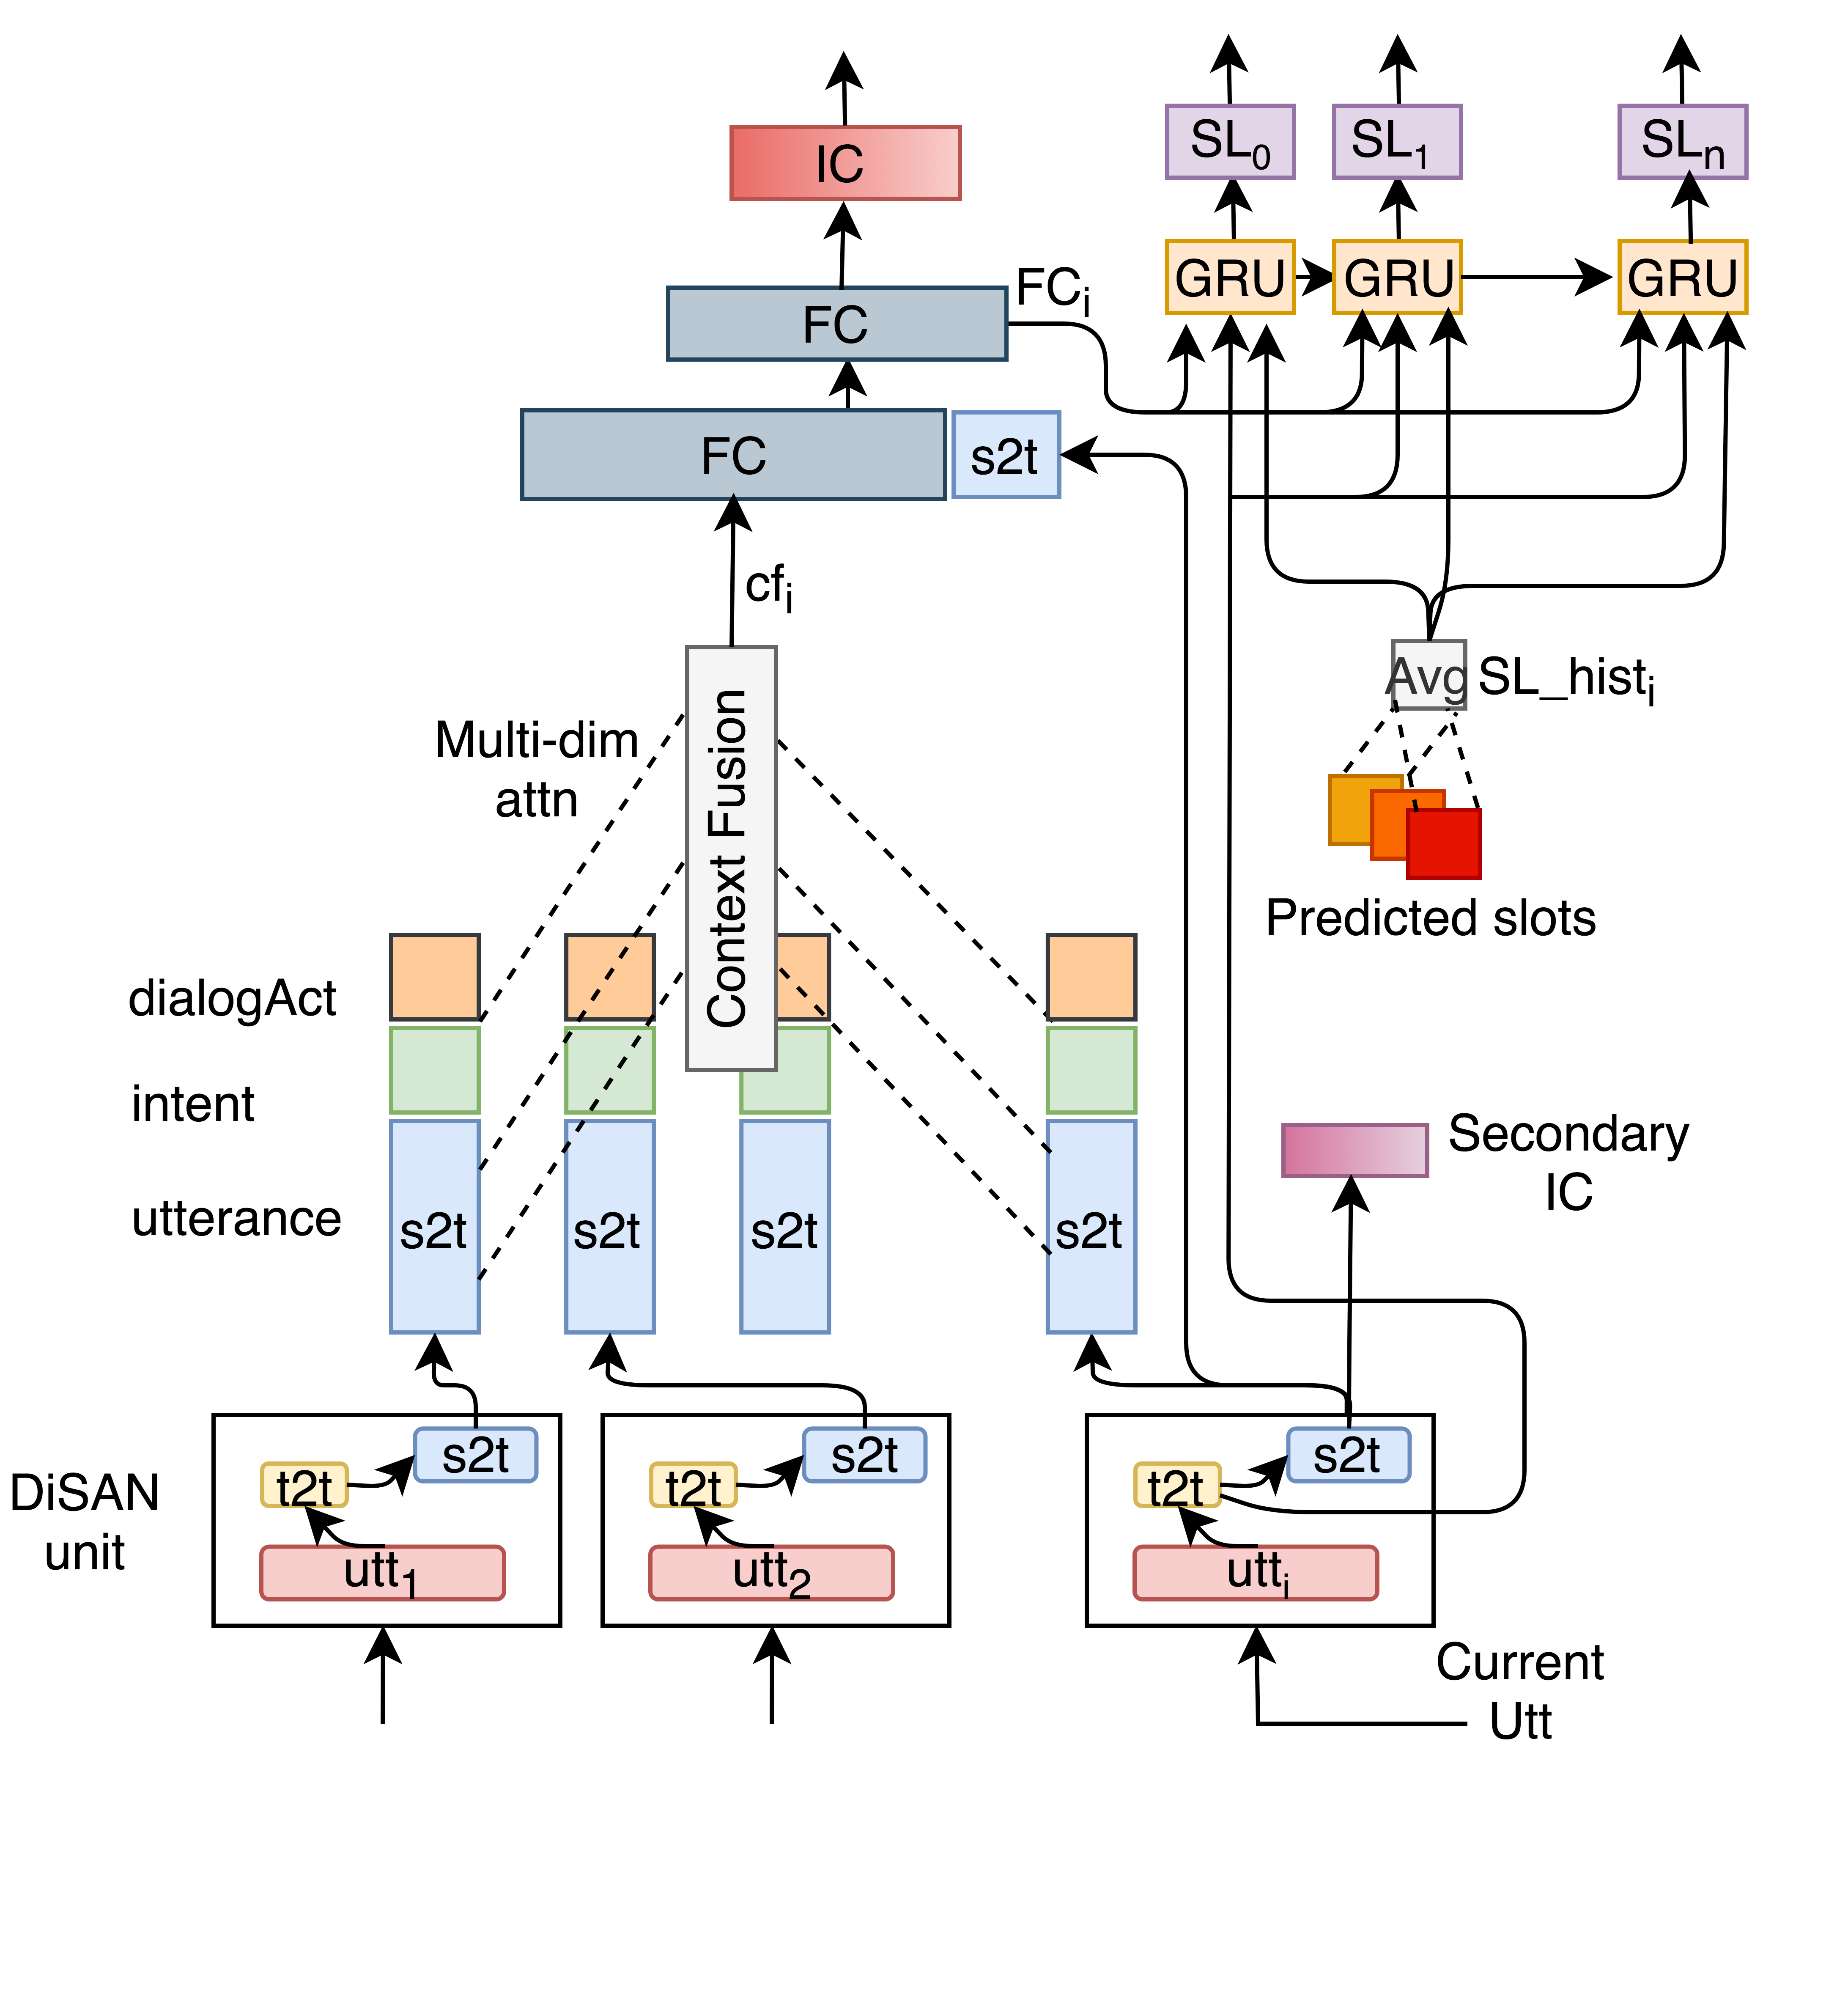
\includegraphics[width=200pt, height=250pt, width=0.5\textwidth]{figures/emnlp_cdisan_cr.png}
\vspace{-50pt}
\caption{\label{cSA} \small \pretty{Casa-nlu} model architecture for joint IC-SL}
\end{figure}
\vspace{-10pt}

\subsection{Signal Encoding}

\textbf{Utterance (Utt):} For the utterance encoding, we adopt the directional self-attention \cite{shen2017disan} based encoder (\pretty{DiSAN}), adding absolute position embedding \cite{gehring2017convolutional} to further improve the encoding performance.\footnote{Details provided in Appendix A}
%To further improve the encoding, we add absolute position embedding \cite{gehring2017convolutional} to the input utterance.
\pretty{DiSAN} unit consists of two types of multi-dimensional attention - word level token2token (t2t) attention followed by sentence level source2token (s2t) attention. For turn $i$, the output of this unit is given by $\h({\text{Utt}}_i) \in\mathbb{R}^{2d_h\times 1}$, 
%where $k_i$ is the utterance length for the $i_{th}$ turn with hidden layer size, $d_h$.
where $d_h$ is hidden layer size of the \pretty{DiSAN} unit (Figure \ref{cSA}).

\noindent \textbf{Intent / Dialog Act (DA) / Slot Label %\footnote{Dialog Act signifies the actions taken by the agent such as Close (when an intent is fulfilled), ConfirmIntent, ElicitSlot, etc}
History:} We pass the one-hot representation of intent ground truth labels through an embedding layer to get intent history representation $\h({\text{I}_i}) \in\mathbb{R}^{d_{I}\times 1}$ for any previous turn $i$ with $d_I$ being the intent embedding dimension. Similarly, for DA history, $\h({\text{DA}_i}) \in\mathbb{R}^{d_{DA}\times 1}$. We use a special dummy symbol for the intent and DA of the current turn.  %We follow a similar procedure for DA.
For slot label history, for turn $i$, we take the average of all slot embeddings that were observed in previous turns giving $\h({\text{SL}\_{\text{hist}}_i}) \in \mathbb{R}^{d_{SL}\times 1}$.
% \arsh{We use ground truth labels as contextual signals in our experiments.}
%%%QUESTION : Clarify what history at i mean ?
%%%Done
\subsection{Context Fusion}
We combine the vectorized signals together in both spacial and temporal dimensions. For the former, we simply concatenate the contextual signals to get current turn feature vector, i.e. ${\mathbf{T}_i} = [\h({\text{Utt}_i});\h({\text{I}_i}); \h({\text{DA}_i})]$. However, for the latter, concatenation %results in a large matrix and might 
becomes intractable if context window is large. To address this issue and automatically learn more relevant components of context for each turn, we %GARIMA adding : compute source2token multi-dimension self attention over each turn vector 
add a source2token \cite{shen2017disan} multi-dimensional self-attention layer over the turn vectors. This is essentially a per dimension learned weighted average ($\mathbf{cf}_i$) over all the turn vectors within a context window (Equation \ref{eq:attn}).
%\st{ per dimension}.
As shown later in Section \ref{sec:results_f}, this enhances the  model's robustness by learning different attention weights for different contextual signals.%  i.e. intent vector could have different attention weights than an utterance vector for the same turn. This enhances the model's robustness. 
%Attention weights, $f(T_i)$ 
%$$f(T_i) = W_1^T\sigma(W_2{T_i} + b_2) + b_1$$
\vspace{-10pt}
\begin{equation}
    \textbf{cf}_i = \sum_{t=i-K}^{i} \textbf{P}(\textbf{T}_t) \odot {\textbf{T}_t} \label{eq:attn}
\end{equation}
\vspace{-10pt}
%$$cf_t = \sum_{i=t-K}^{t} P(T_i) \odot {T_i}$$

\noindent where, $K$ (= 3 in our experiments) is the context window, and $\mathbf{T}_t$ and $\mathbf{P}(\mathbf{T}_t)$ are the turn vector and attention weights for $t^{th}$ time step %in the context window $K$, 
respectively. We use padding tokens for $i-K<0$.

One of the shortcomings with such attention mechanism is that it is position invariant. To address this problem, we add learned absolute position embedding $\textbf{p}_c$ %\in \mathbb{R} 
to the turn matrix $\mathbf{T}$ that learns temporal information across the turns.
%, $\mathbf{T}$ = \textbf{T} + $\textbf{p}_c.$
%\sout{$\mathbf{T}$ := \textbf{T} + $\textbf{p}_c.$}
%\glalwani{$\mathbf{T}_i$ := $\mathbf{T}_i$  + $\textbf{p}_c.$}




\subsection{IC-SL Predictions}
Following \cite{joint_ic_sl, li2018self}, we  train a joint IC-SL model. To improve IC performance for our deep network, we also add a secondary IC loss function, $\text{L}_{\text{Sec}\_\text{IC}}$ at the utterance level (Figure \ref{cSA}). The new aggregated loss is:
% \vspace{-10pt}
\begin{equation}
    \text{L}=\text{L}_{\text{IC}} + \alpha \times \text{L}_{\text{SL}} + \beta \times \text{L}_{\text{Sec}\_\text{IC}}
\end{equation}
% \vspace{5pt}
\textbf{IC:} At turn $i$, we take the output of context fusion layer $\mathbf{cf}_i$, pass it through a fully connected layer and concatenate the output with the current utterance encoding $\h({\text{Utt}_i})$. 
% $$h_{cf_t} = <\sigma(Wcf_t + b);h_{Utt_t}>$$
This is then further projected down using a fully connected layer ($\text{FC}_i$) and finally fed into  \emph{softmax} layer to predict the intent.
\newline


% $$P_{Intent_i}(\cdot)=softmax(W_ih_{cf_t} + b)$$
% where, $i \in (0, num\_intent\_classes)$


\noindent\textbf{SL:} For turn $i$, the t2t attention output is first fused with the utterance embedding using a fusion gate \cite{hochreiter1997long} to generate $\h_{ij}$ where $j$ represents token index in the utterance. 
Then, for each token position in the utterance,
we apply a sliding window, $w$ (=3) over neighboring words
%word context window of size $p$ (=3) is applied 
that transforms each token's embedding space from $\h_{ij}$ to $w \times \h_{ij}$ (not shown in the Figure \ref{cSA}). 
%where $h_{ij}$ represents $j^{\text{th}}$ token's embedding for turn $i$. 
To add contextual information to SL task, each token's dimension is augmented using slot history ($\text{SL}\_\text{hist}_{i}$)  as well as penultimate fully connected layer for IC task ($\text{FC}_i$), yielding a final dimension of $w \times \h_{ij} +  \h({\text{SL}\_{\text{hist}}_i}) +   \h({\text{FC}_i})$. Finally, a Gated Recurrent Unit (GRU) renders the labels auto-regressive followed by \emph{softmax} layer.
%% Arsh you experimented with a CRF layer as well, right? was this worse than using softmax? Arsh: Never experimented with CRF
%% Arsh, where is the elicit slot type passed incorporated in the model? Also I don't see mention of the SL constraints? is this not in scope for this work? Arsh: Not used for this paper as we want to keep it separate from lex's business logic

